\documentclass[%
a4paper,
%twoside,
11pt
]{article}

% encoding, font, language
\usepackage[utf8]{inputenc}
\usepackage[T1]{fontenc}
\usepackage[ngerman, english]{babel}


\usepackage[
    handwritten,
    nowarnings,
    %myconfig
]
{xcookybooky}


\begin{document}

\title{Architecture logicielle \\ Feuille 4 \\ Stratégie temps réel – Armée}
\author{Benoit Barthes - Anne-laure Mesure}
\maketitle

L'objectif de ce TP est d'implémenter à partir de notre structure existante, la notion d'armée. Une armée peut-être composée d'une armée, elle-même composée d'une armée et ainsi de suite.

 \newpage
\section*{Exercice 1}

Dans une premier temps, afin de séparer la partie client de l'implémentation, nous avons eu recours au pattern façade. Nous avons donc créé un nouvelle interface: ISoldierFacade qui comme la classe ISoldierComponent créé lors du tp précédent hérite de l'interface ISoldier.

\begin{figure}[!ht]
    \center
    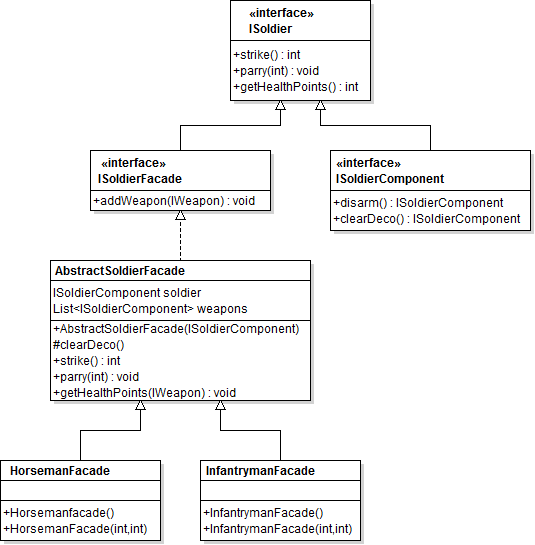
\includegraphics[width =13cm]{imgs/facade.png}
    %\caption{Diagramme UML avant refactoring}
    %\label{bloghiko}
\end{figure}

La façade est testé avec les tests unitaires FullHands qui teste qu'un soldat ne peut avoir plus de deux armes, Parry, qui teste la méthode parry avec un soldat sans équipements puis avec un soldat équipé d'un bouclier, et Strike qui vérifie la méthode strike avec un soldat non armé et un soldat armé.


Dans un deuxième temps, nous avons représenté notre armée à l'aide du pattern Composite, pattern nous permettant de représenter une architecture d'ensembles avec une relation composant/composé.

\begin{figure}[!ht]
    \center
    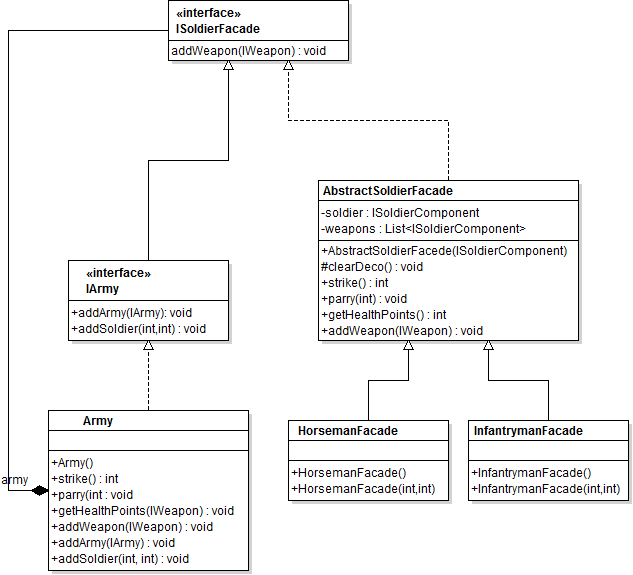
\includegraphics[width =13cm]{imgs/Composite.png}
    %\caption{Diagramme UML avant refactoring}
    %\label{bloghiko}
\end{figure}

Pour tester cette partie de l'implémentation, nous avons créé le fichier de tests unitaires ArmyTest, qui crée un Infantryman et une armée composée d'un Infantryman et on teste s'ils ont le même comportement, puis crée une armée de n soldats et qui vérifie si son nombre de points de vie de l'armée équivaut au nombre de points de vie de n soldats puis si elle comportement de l'armée après un strike ou un parry est cohérent. Dans le dernie test, on vérifie qu'une armée vide à qui on donne une épée ne fasse pas de dégâts.

\section*{Exercice 2}
Cet exercice nous avait pour but de trouver un moyen d'ajouter simplement de nouvelles fonctionnalités sans avoir à l'implémenter dans toutes classes sur lesquels elle agit.
Pour cela nous avons implémenté la méthode accept(Visitor v) dans les classes Army, InfantrymanFacade et HorsemanFacade, méthode accessible depuis l'interface ISoldierFacade.
\newpage

\begin{figure}[!ht]
    \center
    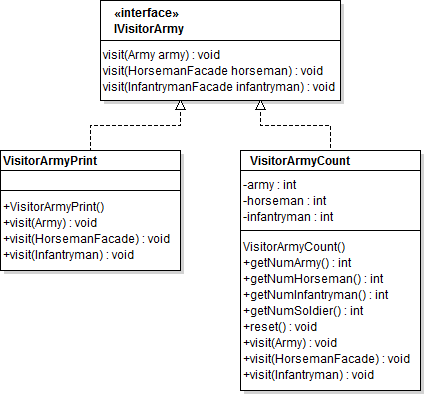
\includegraphics[width = 10cm]{imgs/Visitor.png}
    %\caption{Diagramme UML avant refactoring}
    %\label{bloghiko}
\end{figure}

Pour tester cet implémentation, nous avons créé un fichier de tests TestVisitorCount qui crée une armée et compte ses effectifs, puis crée une seconde armée dans la première et encore une fois compte ses effectifs. Enfin le dernier test crée une armée, crée à l'intérieur des armées vides et vérifie que le compteur reste à 0.

\end{document} 